% This file was created by matlab2tikz.
%
%The latest updates can be retrieved from
%  http://www.mathworks.com/matlabcentral/fileexchange/22022-matlab2tikz-matlab2tikz
%where you can also make suggestions and rate matlab2tikz.
%
\documentclass[tikz]{standalone}
\usepackage[T1]{fontenc}
\usepackage[utf8]{inputenc}
\usepackage{pgfplots}
\usepackage{grffile}
\pgfplotsset{compat=newest}
\usetikzlibrary{plotmarks}
\usepgfplotslibrary{patchplots}
\usepackage{amsmath}

\begin{document}
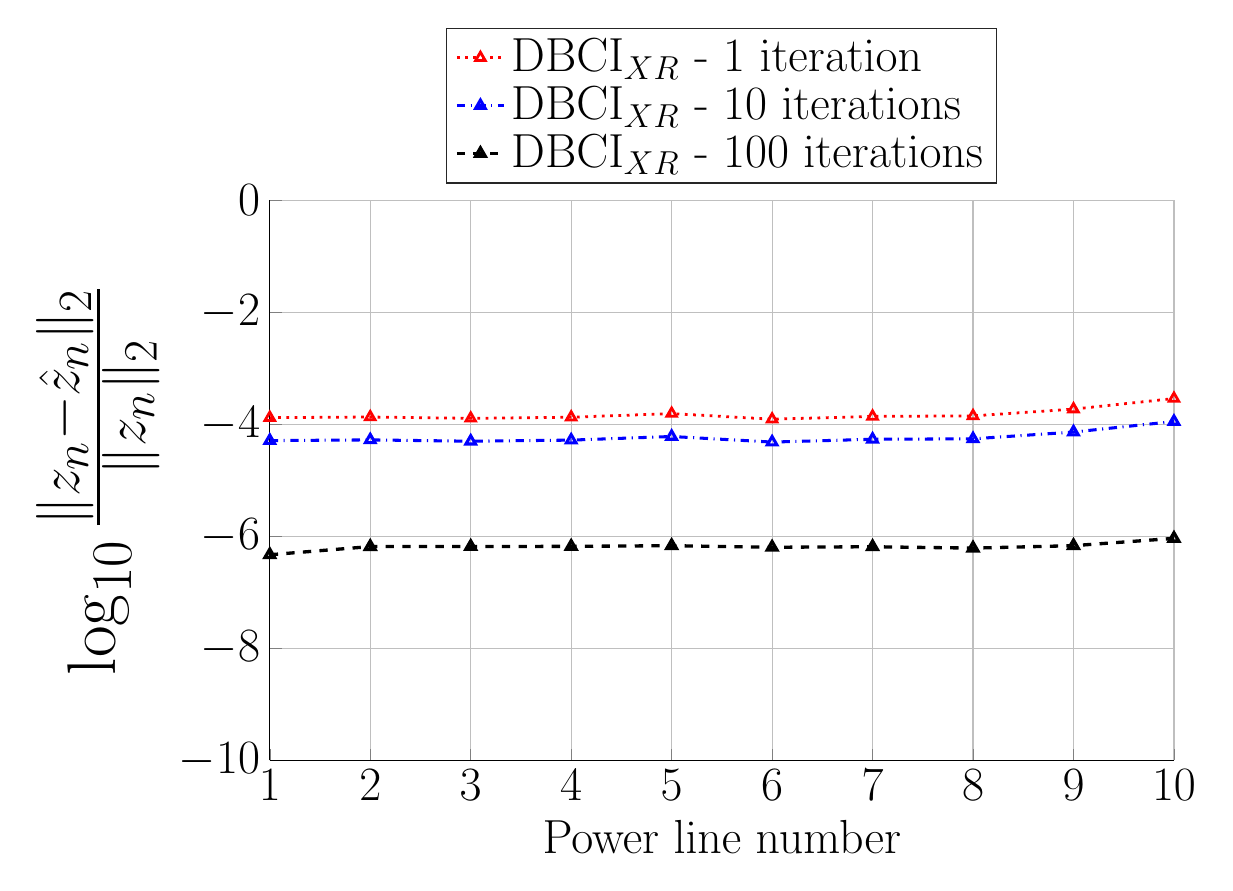
\begin{tikzpicture}

\begin{axis}[%
width=4.521in,
height=2.8in,
at={(0.758in,0.428in)},
scale only axis,
xmin=1,
xmax=10,
xlabel={Power line number},
xmajorgrids,
ymin=-10,
ymax=0,
ylabel={$\log_{10}\frac{\|z_n - \hat{z}_n\|_2}{\|z_n\|_2}$},
ymajorgrids,
axis background/.style={fill=white},
axis x line*=bottom,
axis y line*=left,
legend style={at={(0.5,1.03)},anchor=south,legend cell align=left,align=left,draw=white!15!black},
xlabel style={font=\LARGE},ylabel style={font=\Huge},legend style={font=\LARGE},ticklabel style={font=\LARGE}
]

\addplot [color=red,dotted,line width=1.0pt,mark=triangle,mark options={solid}]
  table[row sep=crcr]{%
1	-3.88090534345849\\
2	-3.86964700560886\\
3	-3.89331250305145\\
4	-3.8735781693953\\
5	-3.80841453476826\\
6	-3.9087658497897\\
7	-3.85832000821522\\
8	-3.84983152727818\\
9	-3.7284474352639\\
10	-3.53956216259043\\
};
\addlegendentry{DBCI$_{XR}$ - 1 iteration};

\addplot [color=blue,dashdotted,line width=1.1pt,mark=triangle,mark options={solid}]
  table[row sep=crcr]{%
1	-4.2904174938234\\
2	-4.2782761821511\\
3	-4.3017398517945\\
4	-4.28214763461237\\
5	-4.21739012037145\\
6	-4.31717221726016\\
7	-4.26705948823946\\
8	-4.25880740157296\\
9	-4.1379507097733\\
10	-3.94946741399456\\
};
\addlegendentry{DBCI$_{XR}$ - 10 iterations};

\addplot [color=black,dashed,line width=1.2pt,mark=triangle,mark options={solid}]
  table[row sep=crcr]{%
1	-6.32939409637337\\
2	-6.1831584219856\\
3	-6.18189088210376\\
4	-6.17946507361347\\
5	-6.16732048573507\\
6	-6.1952229482674\\
7	-6.18612232114627\\
8	-6.21054085497848\\
9	-6.16700097486536\\
10	-6.03675702928428\\
};
\addlegendentry{DBCI$_{XR}$ - 100 iterations};

\end{axis}
\end{tikzpicture}%
\end{document}